\section{向量场在曲线上的积分}

\begin{problem}{第二型曲线积分}{Line-Integral-Type-II}
    计算下列第二型曲线积分：
    \begin{enumerate}
        \item $\int_L (x^2 + y^2) \d x + (x^2 - y^2) \d y$，其中 $L$ 是曲线 $y = 1 - |1 - x|$ 从点 $(0,0)$ 到点 $(2,0)$；
        \item $\int_L \frac{\d x + \d y}{|x| + |y|}$，其中 $L$ 是沿正方形 $A(1,0)$、$B(0,1)$、$C(-1,0)$、$D(0,-1)$ 逆时针一周的路径；
        \item $\int_L \frac{-x \d x + y \d y}{x^2 + y^2}$，其中 $L$ 是圆周 $x^2 + y^2 = a^2$，依逆时针方向一周的路径；
        \item $\int_L y^2 \d x + xy \d y + xz \d z$，其中 $L$ 是从 $O(0,0,0)$ 到 $A(1,0,0)$ 再到 $B(1,1,0)$ 最后到 $C(1,1,1)$ 的折线段；
        \item $\int_L \e^{x+y+z} \d x + \e^{x+y+z} \d y + \e^{x+y+z} \d z$，其中 $L$ 是 $x = \cos \varphi$、$y = \sin \varphi$、$z = \frac{\varphi}{\uppi}$ 从点 $A(1,0,0)$ 到点 $B(0,1,\frac{1}{2})$；
        \item $\int_L y \d x + z \d y + x \d z$，其中 $L$ 是 $x + y = 2$ 与 $x^2 + y^2 + z^2 = 2(x + y)$ 的交线，从原点看去是顺时针方向．
    \end{enumerate}
\end{problem}

\begin{solution}
    \ansitem{1}
    采用分段积分法．

    曲线 $L$ 可表示为：
    \begin{equation}
        y = \begin{cases} x, & 0 \le x \le 1, \\ 2 - x, & 1 \le x \le 2. \end{cases}
    \end{equation}
    记 $L_1$ 为从 $(0,0)$ 到 $(1,1)$ 的线段，$L_2$ 为从 $(1,1)$ 到 $(2,0)$ 的线段．则有
    \begin{equation}
        \begin{aligned}
            \int_{L_1} (x^2 + y^2) \d x + (x^2 - y^2) \d y & = \int_0^1 [x^2 + x^2 + (x^2 - x^2)] \d x = \int_0^1 2x^2 \d x = \frac{2}{3},    \\
            \int_{L_2} (x^2 + y^2) \d x + (x^2 - y^2) \d y & = \int_1^2 [(x^2 + (2-x)^2) \d x + (x^2 - (2-x)^2) (-\d x)]                      \\
                                                           & = \int_1^2 2(2-x)^2 \d x = \left[ -\frac{2}{3}(2-x)^3 \right]_1^2 = \frac{2}{3}.
        \end{aligned}
    \end{equation}
    故原积分为
    \begin{equation}
        I = \boxed{\frac{4}{3}}
    \end{equation}

    \ansitem{2}
    采用分段积分法．

    正方形各边方程分别为：$AB: x+y=1$；$BC: -x+y=1$；$CD: -x-y=1$；$DA: x-y=1$．在各边上均有 $|x|+|y|=1$．
    \begin{equation}
        \begin{aligned}
            \int_{AB} \frac{\d x + \d y}{1} & = \int_1^0 (\d x - \d x) = 0,     \\
            \int_{BC} \frac{\d x + \d y}{1} & = \int_0^{-1} (\d x + \d x) = -2, \\
            \int_{CD} \frac{\d x + \d y}{1} & = \int_{-1}^0 (\d x - \d x) = 0,  \\
            \int_{DA} \frac{\d x + \d y}{1} & = \int_0^1 (\d x + \d x) = 2.
        \end{aligned}
    \end{equation}
    故原积分为
    \begin{equation}
        I = \boxed{0}
    \end{equation}

    \ansitem{3}
    采用参数化积分法．

    令 $x = a \cos \theta$、$y = a \sin \theta$，则 $\d x = -a \sin \theta \d \theta$、$\d y = a \cos \theta \d \theta$，其中 $\theta \in [0, 2\uppi]$．
    \begin{equation}
        \begin{aligned}
            \int_L \frac{-x \d x + y \d y}{x^2 + y^2} & = \int_0^{2\uppi} \frac{-a \cos \theta (-a \sin \theta) + a \sin \theta (a \cos \theta)}{a^2} \d \theta \\
                                                      & = \int_0^{2\uppi} 2 \sin \theta \cos \theta \d \theta = \int_0^{2\uppi} \sin 2\theta \d \theta = 0.
        \end{aligned}
    \end{equation}
    故原积分为
    \begin{equation}
        I = \boxed{0}
    \end{equation}

    \ansitem{4}
    采用分段积分法．

    积分路径由三段组成：
    \begin{equation}
        \begin{aligned}
            OA: y=0, z=0, \d y=0, \d z=0, x \in [0, 1] & \implies \int_{OA} = 0,                             \\
            AB: x=1, z=0, \d x=0, \d z=0, y \in [0, 1] & \implies \int_{AB} = \int_0^1 y \d y = \frac{1}{2}, \\
            BC: x=1, y=1, \d x=0, \d y=0, z \in [0, 1] & \implies \int_{BC} = \int_0^1 z \d z = \frac{1}{2}.
        \end{aligned}
    \end{equation}
    故原积分为
    \begin{equation}
        I = \boxed{1}
    \end{equation}

    \ansitem{5}
    利用全微分性质．

    注意到被积表达式为全微分：
    \begin{equation}
        \e^{x+y+z} \d x + \e^{x+y+z} \d y + \e^{x+y+z} \d z = \d (\e^{x+y+z}).
    \end{equation}
    积分与路径无关，仅取决于起点 $A(1,0,0)$ 与终点 $B(0,1,\frac{1}{2})$．
    \begin{equation}
        \int_L \d (\e^{x+y+z}) = \e^{x+y+z} \Big|_{(1,0,0)}^{(0,1,1/2)} = \e^{1+1/2} - \e^1 = \e^{3/2} - \e.
    \end{equation}
    故原积分为
    \begin{equation}
        I = \boxed{\e^{3/2} - \e}
    \end{equation}

    \ansitem{6}
    直接积分法．

    首先确定交线 $L$ 的方程．将球面方程变形为
    \begin{equation}
        (x-1)^2 + (y-1)^2 + z^2 = 2.
    \end{equation}
    将平面方程 $y = 2 - x$ 代入上式，得
    \begin{equation}
        (x-1)^2 + (2-x-1)^2 + z^2 = 2 \implies 2(x-1)^2 + z^2 = 2.
    \end{equation}
    由此可得 $L$ 的参数方程．令 $x - 1 = \cos \theta$，则 $z = \sqrt{2} \sin \theta$．进而由 $y = 2 - x$ 得 $y = 1 - \cos \theta$．即
    \begin{equation}
        \begin{cases}
            x = 1 + \cos \theta, \\
            y = 1 - \cos \theta, \\
            z = \sqrt{2} \sin \theta.
        \end{cases}
    \end{equation}
    对应的微分项为
    \begin{equation}
        \d x = -\sin \theta \d \theta, \quad \d y = \sin \theta \d \theta, \quad \d z = \sqrt{2} \cos \theta \d \theta.
    \end{equation}
    判断方向：当 $\theta$ 从 $0$ 增加到 $\frac{\uppi}{2}$ 时，点从 $(2,0,0)$ 移动到 $(1,1,\sqrt{2})$．从原点 $(0,0,0)$ 观察，该运动方向为逆时针方向．题目要求顺时针方向，故积分范围应为 $\theta \in [2\uppi, 0]$．

    将参数方程代入被积表达式：
    \begin{equation}
        \begin{aligned}
            y \d x + z \d y + x \d z & = (1 - \cos \theta)(-\sin \theta \d \theta) + (\sqrt{2} \sin \theta)(\sin \theta \d \theta) + (1 + \cos \theta)(\sqrt{2} \cos \theta \d \theta) \\
                                     & = \left( -\sin \theta + \sin \theta \cos \theta + \sqrt{2} \sin^2 \theta + \sqrt{2} \cos \theta + \sqrt{2} \cos^2 \theta \right) \d \theta      \\
                                     & = \left( \sqrt{2} + \sqrt{2} \cos \theta - \sin \theta + \frac{1}{2} \sin 2\theta \right) \d \theta.
        \end{aligned}
    \end{equation}
    对上述表达式在 $[2\uppi, 0]$ 上积分：
    \begin{equation}
        \begin{aligned}
            I & = \int_{2\uppi}^0 \left( \sqrt{2} + \sqrt{2} \cos \theta - \sin \theta + \frac{1}{2} \sin 2\theta \right) \d \theta       \\
              & = \left. \left( \sqrt{2}\theta + \sqrt{2} \sin \theta + \cos \theta - \frac{1}{4} \cos 2\theta \right) \right|_{2\uppi}^0 \\
              & = \left( 0 + 0 + 1 - \frac{1}{4} \right) - \left( 2\sqrt{2}\uppi + 0 + 1 - \frac{1}{4} \right)                            \\
              & = -2\sqrt{2}\uppi.
        \end{aligned}
    \end{equation}
    \begin{equation}
        \boxed{\oint_L y \d x + z \d y + x \d z = -2\sqrt{2}\uppi}
    \end{equation}
\end{solution}

\begin{problem}{曲线积分}{Line-Integral}
    求向量场 $\symbfit{v} = (y + z)\symbfit{i} + (z + x)\symbfit{j} + (x + y)\symbfit{k}$ 沿曲线 $L: x = a \sin^2 t$、$y = 2a \sin t \cos t$、$z = a \cos^2 t$ ($0 \le t \le \uppi$) 参数增加方向的曲线积分．
\end{problem}

\begin{solution}
    记向量场 $\symbfit{v} = (P, Q, R)$．由于
    \begin{equation}
        \frac{\partial R}{\partial y} = \frac{\partial Q}{\partial z} = 1, \quad \frac{\partial P}{\partial z} = \frac{\partial R}{\partial x} = 1, \quad \frac{\partial Q}{\partial x} = \frac{\partial P}{\partial y} = 1,
    \end{equation}
    可知 $\operatorname{curl} \symbfit{v} = \symbfit{0}$，即该向量场在全空间内是保守场．

    考察曲线 $L$ 的起点与终点．当 $t = 0$ 时，起点为
    \begin{equation}
        A = (a \sin^2 0, 2a \sin 0 \cos 0, a \cos^2 0) = (0, 0, a).
    \end{equation}
    当 $t = \uppi$ 时，终点为
    \begin{equation}
        B = (a \sin^2 \uppi, 2a \sin \uppi \cos \uppi, a \cos^2 \uppi) = (0, 0, a).
    \end{equation}
    由于起点与终点重合，且保守场的环量为零，设所求积分为 $I$，则有
    \begin{equation}
        \boxed{I = 0}.
    \end{equation}
\end{solution}

\begin{problem}{变力做功}{Work-Done-by-Elastic-Force}
    设一质点处于弹性力场中，弹力方向指向原点，大小与质点离原点的距离成正比，比例系数为 $k$．若质点沿椭圆 $\frac{x^2}{a^2} + \frac{y^2}{b^2} = 1$ 从点 $(a, 0)$ 移到点 $(0, b)$，求弹性力所做的功．
\end{problem}

\begin{solution}
    设质点的位置向量为 $\symbfit{r} = (x, y)$，由题意可知弹性力场为
    \begin{equation}
        \symbfit{F} = -k \symbfit{r} = -k(x \symbfit{i} + y \symbfit{j}).
    \end{equation}
    弹性力所做的功 $W$ 为
    \begin{equation}
        W = \int_L \symbfit{F} \cdot \d \symbfit{r} = \int_{(a, 0)}^{(0, b)} -kx \d x - ky \d y.
    \end{equation}
    由于 $\frac{\partial (-ky)}{\partial x} = \frac{\partial (-kx)}{\partial y} = 0$，该力场是保守场．其势函数可表示为 $U(x, y) = -\frac{1}{2}k(x^2 + y^2)$．根据曲线积分基本定理，有
    \begin{equation}
        \begin{aligned}
            W & = U(0, b) - U(a, 0)                                                  \\
              & = -\frac{1}{2}k(0^2 + b^2) - \left[ -\frac{1}{2}k(a^2 + 0^2) \right] \\
              & = \frac{1}{2}k(a^2 - b^2).
        \end{aligned}
    \end{equation}
    因此，弹性力所做的功为
    \begin{equation}
        \boxed{W = \frac{1}{2}k(a^2 - b^2)}.
    \end{equation}
\end{solution}

\begin{problem}{Green公式}{Green-Formula}
    利用 Green 公式计算下列曲线积分．
    \begin{enumerate}
        \item $\oint_L (x+y)^2 \d x + (x^2-y^2) \d y$，$L$ 是顶点为 $A(1,1)$、$B(3,3)$、$C(3,5)$ 的三角形的周界，沿反时针方向；
        \item $\oint_L (xy+x+y) \d x + (xy+x-y) \d y$，$L$ 是椭圆 $\frac{x^2}{a^2} + \frac{y^2}{b^2} = 1$ 沿顺时针方向；
        \item $\oint_L (y x^3 + \e^y) \d x + (x y^3 + x \e^y - 2y) \d y$，$L$ 是对称于两坐标轴的闭曲线；
        \item $\oint_L \sqrt{x^2+y^2} \d x + y[xy + \ln (x + \sqrt{x^2+y^2})] \d y$，$L$ 是 $y^2 = x-1$ 与 $x=2$ 围成的封闭曲线沿逆时针方向；
        \item $\int_{AMB} (x^2+2xy-y^2) \d x + (x^2-2xy+y^2) \d y$，$L$ 是从点 $A(0,-1)$ 沿直线 $y=x-1$ 到点 $M(1,0)$，再从 $M$ 沿圆周 $x^2+y^2=1$ 到点 $B(0,1)$；
        \item $\int_{AMO} (\e^x \sin y - my) \d x + (\e^x \cos y - m) \d y$，其中 $AMO$ 为由点 $A(a,0)$ 到点 $O(0,0)$ 的上半圆周 $x^2+y^2=ax$ ($a>0$)．
    \end{enumerate}
\end{problem}

\begin{solution}
    \ansitem{1}

    记原曲线积分为 $I$．设 $L$ 围成的内部区域为 $D$，由题意可知 $D$ 为由直线 $y=x$、$y=2x-1$ 与 $x=3$ 围成的闭区域．应用 Green 公式可得
    \begin{equation}
        \begin{aligned}
            I & = \iint_D \left[ \frac{\partial}{\partial x}(x^2-y^2) - \frac{\partial}{\partial y}(x+y)^2 \right] \d x \d y \\
              & = \iint_D [2x - 2(x+y)] \d x \d y                                                                            \\
              & = \iint_D (-2y) \d x \d y.
        \end{aligned}
    \end{equation}
    化为二次积分进行计算，
    \begin{equation}
        \begin{aligned}
            I & = \int_1^3 \d x \int_x^{2x-1} (-2y) \d y      \\
              & = \int_1^3 \left[ -y^2 \right]_x^{2x-1} \d x  \\
              & = \int_1^3 \left( x^2 - (2x-1)^2 \right) \d x \\
              & = \int_1^3 \left( -3x^2 + 4x - 1 \right) \d x \\
              & = \left[ -x^3 + 2x^2 - x \right]_1^3          \\
              & = (-27 + 18 - 3) - (-1 + 2 - 1)               \\
              & = -12.
        \end{aligned}
    \end{equation}
    \begin{equation}
        I = \boxed{-12}.
    \end{equation}

    \ansitem{2}

    设原积分为 $I$，积分区域为 $D = \left\{ (x, y) \mathrel{\big|} \frac{x^2}{a^2} + \frac{y^2}{b^2} \le 1 \right\}$．因曲线 $L$ 沿顺时针方向，应用 Green 公式时需附加负号，
    \begin{equation}
        \begin{aligned}
            I & = -\iint_D \left[ \frac{\partial}{\partial x}(xy+x-y) - \frac{\partial}{\partial y}(xy+x+y) \right] \d x \d y \\
              & = -\iint_D [ (y+1) - (x+1) ] \d x \d y                                                                        \\
              & = \iint_D (x-y) \d x \d y.
        \end{aligned}
    \end{equation}
    积分区域 $D$ 关于原点（以及两坐标轴）对称，而被积函数中的 $x$ 与 $y$ 分别是关于 $x$ 和 $y$ 的奇函数，其在对称区域上的积分皆为零，
    \begin{equation}
        I = \boxed{0}.
    \end{equation}

    \ansitem{3}

    设原积分为 $I$，曲线 $L$ 围成的内部闭区域为 $D$．由 Green 公式可得
    \begin{equation}
        \begin{aligned}
            I & = \iint_D \left[ \frac{\partial}{\partial x}(xy^3+x\e^y-2y) - \frac{\partial}{\partial y}(yx^3+\e^y) \right] \d x \d y \\
              & = \iint_D[ (y^3+\e^y) - (x^3+\e^y) ] \d x \d y                                                                         \\
              & = \iint_D (y^3-x^3) \d x \d y.
        \end{aligned}
    \end{equation}
    根据题意，曲线 $L$ 关于两坐标轴对称，故其围成的区域 $D$ 亦关于两坐标轴对称．被积函数 $y^3-x^3$ 的各分项在对应方向上均为奇函数，积分值必为零，
    \begin{equation}
        I = \boxed{0}.
    \end{equation}

    \ansitem{4}

    设原积分为 $I$，内部闭区域为 $D$．应用 Green 公式可得
    \begin{equation}
        \begin{aligned}
            I & = \iint_D \left\{ \frac{\partial}{\partial x} \left[ y \left( xy + \ln(x+\sqrt{x^2+y^2}) \right) \right] - \frac{\partial}{\partial y}\sqrt{x^2+y^2} \right\} \d x \d y \\
              & = \iint_D \left[ y^2 + y \frac{1+\frac{x}{\sqrt{x^2+y^2}}}{x+\sqrt{x^2+y^2}} - \frac{y}{\sqrt{x^2+y^2}} \right] \d x \d y                                               \\
              & = \iint_D \left[ y^2 + \frac{y}{\sqrt{x^2+y^2}} - \frac{y}{\sqrt{x^2+y^2}} \right] \d x \d y                                                                            \\
              & = \iint_D y^2 \d x \d y.
        \end{aligned}
    \end{equation}
    区域 $D$ 由 $y^2 = x-1$ 与 $x = 2$ 围成，化简得 $y^2 + 1 \le x \le 2$，从而 $y \in [-1, 1]$．化为二次积分，
    \begin{equation}
        \begin{aligned}
            I & = \int_{-1}^1 \d y \int_{y^2+1}^2 y^2 \d x        \\
              & = \int_{-1}^1 y^2 \left( 2 - (y^2+1) \right) \d y \\
              & = \int_{-1}^1 (y^2-y^4) \d y                      \\
              & = 2 \int_0^1 (y^2-y^4) \d y                       \\
              & = 2 \left( \frac{1}{3} - \frac{1}{5} \right)      \\
              & = \frac{4}{15}.
        \end{aligned}
    \end{equation}
    \begin{equation}
        I = \boxed{\frac{4}{15}}.
    \end{equation}

    \ansitem{5}

    记 $P = x^2+2xy-y^2$，$Q = x^2-2xy+y^2$，计算其偏导数得
    \begin{equation}
        \frac{\partial Q}{\partial x} = 2x-2y, \quad \frac{\partial P}{\partial y} = 2x-2y.
    \end{equation}
    为应用 Green 公式，补充有向直线段 $L_{BA}$，其起于 $B(0,1)$ 并沿 $y$ 轴直达 $A(0,-1)$．原路径 $L_{AMB}$ 与 $L_{BA}$ 拼接形成闭曲线 $C = L_{AMB} + L_{BA}$．设其所围成的内部区域为 $D$，由 Green 公式可得
    \begin{equation}
        \oint_C P \d x + Q \d y = \iint_D \left( \frac{\partial Q}{\partial x} - \frac{\partial P}{\partial y} \right) \d x \d y = \iint_D 0 \d x \d y = 0.
    \end{equation}
    故原积分可转化为沿线段 $L_{AB}$（由 $A(0,-1)$ 到 $B(0,1)$）的积分．在路径 $L_{AB}$ 上，参数方程为 $x=0$ 且 $y$ 从 $-1$ 到 $1$，从而 $\d x = 0$．代入计算得
    \begin{equation}
        \begin{aligned}
            \int_{AMB} P \d x + Q \d y & = \int_{L_{AB}} P \d x + Q \d y        \\
                                       & = \int_{-1}^1 Q(0,y) \d y              \\
                                       & = \int_{-1}^1 y^2 \d y                 \\
                                       & = \left[ \frac{1}{3}y^3 \right]_{-1}^1 \\
                                       & = \frac{2}{3}.
        \end{aligned}
    \end{equation}
    \begin{equation}
        \int_{AMB} P \d x + Q \d y = \boxed{\frac{2}{3}}.
    \end{equation}

    \ansitem{6}

    记 $P = \e^x \sin y - my$，$Q = \e^x \cos y - m$．
    原曲线 $L_{AMO}$ 不是闭曲线．补充有向线段 $L_{OA}$（沿 $x$ 轴从 $O(0,0)$ 到 $A(a,0)$），与 $L_{AMO}$ 共同构成逆时针闭曲线 $C = L_{OA} + L_{AMO}$．设其围成的半圆区域为 $D$，应用 Green 公式可得
    \begin{equation}
        \begin{aligned}
            \oint_C P \d x + Q \d y & = \iint_D \left[ \frac{\partial}{\partial x}(\e^x \cos y - m) - \frac{\partial}{\partial y}(\e^x \sin y - my) \right] \d x \d y \\
                                    & = \iint_D \left( \e^x \cos y - \e^x \cos y + m \right) \d x \d y                                                                \\
                                    & = m \iint_D \d x \d y.
        \end{aligned}
    \end{equation}
    区域 $D$ 是半径为 $\frac{a}{2}$ 的半圆，其面积为 $\frac{1}{2} \uppi \left(\frac{a}{2}\right)^2 = \frac{\uppi a^2}{8}$．因而
    \begin{equation}
        \label{eq:green-6-1}
        \oint_C P \d x + Q \d y = \frac{\uppi a^2 m}{8}.
    \end{equation}
    对于辅助线段 $L_{OA}$，路径方程为 $y=0$ 且 $x \in [0, a]$，故 $\d y = 0$．计算沿此路径的积分，
    \begin{equation}
        \label{eq:green-6-2}
        \int_{L_{OA}} P \d x + Q \d y = \int_0^a (\e^x \sin 0 - m \cdot 0) \d x = 0.
    \end{equation}
    结合\zcref{eq:green-6-1}与\zcref{eq:green-6-2}可得原积分值为
    \begin{equation}
        \begin{aligned}
            \int_{L_{AMO}} P \d x + Q \d y & = \oint_C P \d x + Q \d y - \int_{L_{OA}} P \d x + Q \d y \\
                                           & = \frac{\uppi a^2 m}{8} - 0.
        \end{aligned}
    \end{equation}
    \begin{equation}
        \int_{L_{AMO}} P \d x + Q \d y = \boxed{\frac{\uppi a^2 m}{8}}.
    \end{equation}
\end{solution}

\begin{problem}{曲线积分求面积}{Line-Integral-Area}
    利用曲线积分计算下列区域的面积．
    \begin{enumerate}
        \item 星形线 $x = a \cos^3 t, y = a \sin^3 t$ ($0 \le t \le 2\uppi$) 围成的区域；
        \item 旋轮线 $x = a(t - \sin t), y = a(1 - \cos t)$ ($0 \le t \le 2\uppi$) 与 $Ox$ 轴所围成的区域．
    \end{enumerate}
\end{problem}

\begin{solution}
    \ansitem{1}

    \begin{center}
        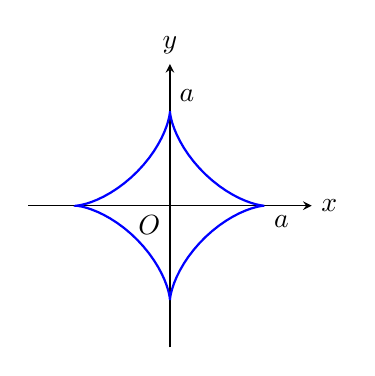
\begin{tikzpicture}[scale=1.2, >=stealth]
            \draw[->] (-1.5,0) -- (1.5,0) node[right] {$x$};
            \draw[->] (0,-1.5) -- (0,1.5) node[above] {$y$};
            \draw[thick, blue, domain=0:2*pi, samples=100] plot ({cos(\x r)^3}, {sin(\x r)^3});
            \node at (1,0) [below right] {$a$};
            \node at (0,1) [above right] {$a$};
            \node at (0,0) [below left] {$O$};
        \end{tikzpicture}
    \end{center}
    由面积公式 $A = \frac{1}{2} \oint_L x \d y - y \d x$．对星形线有
    \begin{equation}\label{eq:astroid-diff}
        \begin{aligned}
            \d x & = -3a \cos^2 t \sin t \d t, \\
            \d y & = 3a \sin^2 t \cos t \d t.
        \end{aligned}
    \end{equation}
    代入公式得
    \begin{equation}\label{eq:astroid-calc}
        \begin{aligned}
            A & = \frac{1}{2} \int_0^{2\uppi} \left[ (a \cos^3 t)(3a \sin^2 t \cos t) - (a \sin^3 t)(-3a \cos^2 t \sin t) \right] \d t \\
              & = \frac{3a^2}{2} \int_0^{2\uppi} (\cos^4 t \sin^2 t + \sin^4 t \cos^2 t) \d t                                          \\
              & = \frac{3a^2}{2} \int_0^{2\uppi} \sin^2 t \cos^2 t (\cos^2 t + \sin^2 t) \d t                                          \\
              & = \frac{3a^2}{8} \int_0^{2\uppi} \sin^2 2t \d t                                                                        \\
              & = \frac{3a^2}{16} \int_0^{2\uppi} (1 - \cos 4t) \d t = \frac{3}{8} \uppi a^2.
        \end{aligned}
    \end{equation}
    \begin{equation}
        A = \boxed{\frac{3}{8} \uppi a^2}
    \end{equation}

    \ansitem{2}

    \begin{center}
        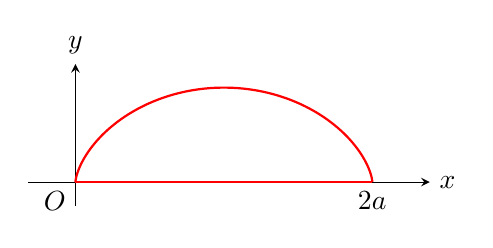
\begin{tikzpicture}[scale=0.6, >=stealth]
            \draw[->] (-1,0) -- (7.5,0) node[right] {$x$};
            \draw[->] (0,-0.5) -- (0,2.5) node[above] {$y$};
            \draw[thick, red, domain=0:2*pi, samples=100] plot ({\x - sin(\x r)}, {1 - cos(\x r)});
            \draw[thick, red] (0,0) -- (6.28,0);
            \node at (6.28,0) [below] {$2\uppi a$};
            \node at (0,0) [below left] {$O$};
        \end{tikzpicture}
    \end{center}
    边界由旋轮线弧 $L_1$ 与 $x$ 轴线段 $L_2$ 组成．在 $L_2$ 上 $y=0$，取顺时针方向围成的面积为
    \begin{equation}\label{eq:cycloid-calc}
        \begin{aligned}
            A & = \int_0^{2\uppi} y(t) x'(t) \d t                                                         \\
              & = \int_0^{2\uppi} a(1 - \cos t) \cdot a(1 - \cos t) \d t                                  \\
              & = a^2 \int_0^{2\uppi} (1 - 2\cos t + \cos^2 t) \d t                                       \\
              & = a^2 \int_0^{2\uppi} \left( 1 - 2\cos t + \frac{1 + \cos 2t}{2} \right) \d t             \\
              & = a^2 \left[ \frac{3}{2}t - 2\sin t + \frac{1}{4}\sin 2t \right]_0^{2\uppi} = 3\uppi a^2.
        \end{aligned}
    \end{equation}
    \begin{equation}
        A = \boxed{3\uppi a^2}
    \end{equation}
\end{solution}

\begin{problem}{全微分与曲线积分}{Line-Integral-Differential-Form}
    计算曲线积分 $\int_{L} \frac{-y \d x + x \d y}{x^2 + y^2}$.
    \begin{enumerate}
        \item $L$ 为从点 $A(-a, 0)$ 沿圆周 $y = \sqrt{a^2 - x^2}$ 到点 $B(a, 0), a > 0$;
        \item $L$ 为从点 $A(-1, 0)$ 沿抛物线 $y = 4 - (x - 1)^2$ 到点 $B(3, 0)$.
    \end{enumerate}
\end{problem}

\begin{solution}
    \ansitem{1}

    记 $P(x, y) = \frac{-y}{x^2 + y^2}, Q(x, y) = \frac{x}{x^2 + y^2}$．在不包含原点的单连通区域内，由于
    \begin{equation}
        \label{eq:partial-derivatives}
        \frac{\partial Q}{\partial x} = \frac{y^2 - x^2}{(x^2 + y^2)^2}, \quad \frac{\partial P}{\partial y} = \frac{y^2 - x^2}{(x^2 + y^2)^2}
    \end{equation}
    可知 $\frac{\partial Q}{\partial x} = \frac{\partial P}{\partial y}$．注意到该微分形式恰为极角 $\theta$ 的全微分，即
    \begin{equation}
        \d \theta = \d \left( \arctan \frac{y}{x} \right) = \frac{-y \d x + x \d y}{x^2 + y^2}
    \end{equation}
    对于上半圆周 $L$，其起点 $A(-a, 0)$ 对应的极角 $\theta_A = \uppi$，终点 $B(a, 0)$ 对应的极角 $\theta_B = 0$．故积分值为
    \begin{equation}
        \int_L \frac{-y \d x + x \d y}{x^2 + y^2} = \int_{\uppi}^0 \d \theta = 0 - \uppi = -\uppi
    \end{equation}
    \begin{equation}
        \boxed{I = -\uppi}
    \end{equation}

    \ansitem{2}

    对于抛物线 $y = 4 - (x - 1)^2$，当 $x \in [-1, 3]$ 时，$y \ge 0$．该路径位于上半平面且不经过原点 $(0,0)$．
    根据曲线积分与路径无关的性质，从 $A(-1, 0)$ 到 $B(3, 0)$ 且不经过原点的路径积分值仅取决于起止点的极角．
    由于起点 $A(-1, 0)$ 的极角 $\theta_A = \uppi$，终点 $B(3, 0)$ 的极角 $\theta_B = 0$，且路径位于上半平面，其角度改变量为
    \begin{equation}
        \Delta \theta = \theta_B - \theta_A = 0 - \uppi = -\uppi
    \end{equation}
    因此，该曲线积分的结果为
    \begin{equation}
        \boxed{I = -\uppi}
    \end{equation}
\end{solution}

\begin{problem}{Green 公式与 Laplace 算子}{Green-Formula-Laplace}
    设 $D$ 是平面上由简单闭曲线 $L$ 围成的区域．
    \begin{enumerate}
        \item 如果 $f(x,y)$ 有连续的二阶导数，证明 $\oint_{L} \frac{\partial f}{\partial \symbfit{n}} \d s = \iint_{D} \Delta f \d x \d y$，这里 $\symbfit{n}$ 是曲线 $L$ 的单位外法向量，$\Delta = \frac{\partial^2}{\partial x^2} + \frac{\partial^2}{\partial y^2}$ 称为二维的 Laplace 算子．因此，当 $f$ 满足 Laplace 方程 $\Delta f = 0$ 时，有 $\oint_{L} \frac{\partial f}{\partial \symbfit{n}} \d s = 0$．（提示：设单位外法向量为 $\symbfit{n} = \cos \alpha \symbfit{i} + \cos \beta \symbfit{j}$，则平面曲线 $L$ 指向逆时针方向的单位切向量为 $\symbfit{\tau} = -\cos \beta \symbfit{i} + \cos \alpha \symbfit{j}$）．
        \item 如果 $\symbfit{a}$ 是单位常值向量，证明：$\oint_{L} \cos(\symbfit{a}, \symbfit{n}) \d s = 0$．
        \item 如果 $u(x,y), v(x,y)$ 有连续的二阶导数，证明下列第二 Green 公式：
              \begin{equation}
                  \oint_{L} \left( v \frac{\partial u}{\partial \symbfit{n}} - u \frac{\partial v}{\partial \symbfit{n}} \right) \d s = \iint_{D} (v \Delta u - u \Delta v) \d x \d y.
              \end{equation}
    \end{enumerate}
\end{problem}

\begin{myproof}
    \ansitem{1} 证明如下．

    设 $L$ 的参数方程为 $x = x(s)$、$y = y(s)$，其中 $s$ 为弧长参数．由提示可知，单位切向量 $\symbfit{\tau} = \left( \frac{\d x}{\d s}, \frac{\d y}{\d s} \right) = (-\cos \beta, \cos \alpha)$．由此可得
    \begin{equation}\label{eq:normal-relation}
        \cos \alpha = \frac{\d y}{\d s}, \quad \cos \beta = -\frac{\d x}{\d s}.
    \end{equation}
    根据方向导数与梯度的关系，有
    \begin{equation}\label{eq:directional-derivative}
        \begin{aligned}
            \oint_{L} \frac{\partial f}{\partial \symbfit{n}} \d s & = \oint_{L} (\nabla f \cdot \symbfit{n}) \d s                                                                         \\
                                                                   & = \oint_{L} \left( \frac{\partial f}{\partial x} \cos \alpha + \frac{\partial f}{\partial y} \cos \beta \right) \d s.
        \end{aligned}
    \end{equation}
    将 \zcref{eq:normal-relation} 代入 \zcref{eq:directional-derivative}，并利用 Green 公式得
    \begin{equation}
        \begin{aligned}
            \oint_{L} \frac{\partial f}{\partial \symbfit{n}} \d s & = \oint_{L} \left( \frac{\partial f}{\partial x} \frac{\d y}{\d s} - \frac{\partial f}{\partial y} \frac{\d x}{\d s} \right) \d s                                                         \\
                                                                   & = \oint_{L} -\frac{\partial f}{\partial y} \d x + \frac{\partial f}{\partial x} \d y                                                                                                      \\
                                                                   & = \iint_{D} \left[ \frac{\partial}{\partial x} \left( \frac{\partial f}{\partial x} \right) - \frac{\partial}{\partial y} \left( -\frac{\partial f}{\partial y} \right) \right] \d x \d y \\
                                                                   & = \iint_{D} \left( \frac{\partial^2 f}{\partial x^2} + \frac{\partial^2 f}{\partial y^2} \right) \d x \d y.
        \end{aligned}
    \end{equation}
    由 Laplace 算子的定义，即证得
    \begin{equation}
        \boxed{\oint_{L} \frac{\partial f}{\partial \symbfit{n}} \d s = \iint_{D} \Delta f \d x \d y}
    \end{equation}

    \ansitem{2} 证明如下．

    由于 $\symbfit{a}$ 与 $\symbfit{n}$ 均为单位向量，故 $\cos(\symbfit{a}, \symbfit{n}) = \symbfit{a} \cdot \symbfit{n}$．设 $\symbfit{a} = a_1 \symbfit{i} + a_2 \symbfit{j}$ 为常向量，则
    \begin{equation}
        \begin{aligned}
            \oint_{L} \cos(\symbfit{a}, \symbfit{n}) \d s & = \oint_{L} (a_1 \cos \alpha + a_2 \cos \beta) \d s \\
                                                          & = \oint_{L} (a_1 \d y - a_2 \d x).
        \end{aligned}
    \end{equation}
    再次运用 Green 公式，由于 $a_1$、$a_2$ 为常数，其偏导数为零，故有
    \begin{equation}
        \oint_{L} a_1 \d y - a_2 \d x = \iint_{D} \left( \frac{\partial a_1}{\partial x} + \frac{\partial a_2}{\partial y} \right) \d x \d y = 0.
    \end{equation}
    即证得
    \begin{equation}
        \boxed{\oint_{L} \cos(\symbfit{a}, \symbfit{n}) \d s = 0}
    \end{equation}

    \ansitem{3} 证明如下．

    考虑向量场 $\symbfit{F} = v \nabla u$．由散度定理可知
    \begin{equation}\label{eq:first-green-prep}
        \oint_{L} v \frac{\partial u}{\partial \symbfit{n}} \d s = \oint_{L} (v \nabla u) \cdot \symbfit{n} \d s = \iint_{D} \operatorname{div} (v \nabla u) \d x \d y.
    \end{equation}
    利用恒等式 $\operatorname{div} (v \nabla u) = \nabla v \cdot \nabla u + v \Delta u$，代入 \zcref{eq:first-green-prep} 得
    \begin{equation}\label{eq:first-green}
        \oint_{L} v \frac{\partial u}{\partial \symbfit{n}} \d s = \iint_{D} (\nabla u \cdot \nabla v + v \Delta u) \d x \d y.
    \end{equation}
    同理，交换 $u$、$v$ 的角色可得
    \begin{equation}\label{eq:first-green-alt}
        \oint_{L} u \frac{\partial v}{\partial \symbfit{n}} \d s = \iint_{D} (\nabla v \cdot \nabla u + u \Delta v) \d x \d y.
    \end{equation}
    将 \zcref{eq:first-green} 与 \zcref{eq:first-green-alt} 相减，即得
    \begin{equation}
        \boxed{\oint_{L} \left( v \frac{\partial u}{\partial \symbfit{n}} - u \frac{\partial v}{\partial \symbfit{n}} \right) \d s = \iint_{D} (v \Delta u - u \Delta v) \d x \d y}
    \end{equation}
\end{myproof}

\endinput
